\documentclass[tikz,convert={outfile=.png}]{standalone}


\usepackage{tikz}
\usetikzlibrary{shapes,backgrounds,calc,patterns}
\usepackage{venndiagram}


\begin{document}
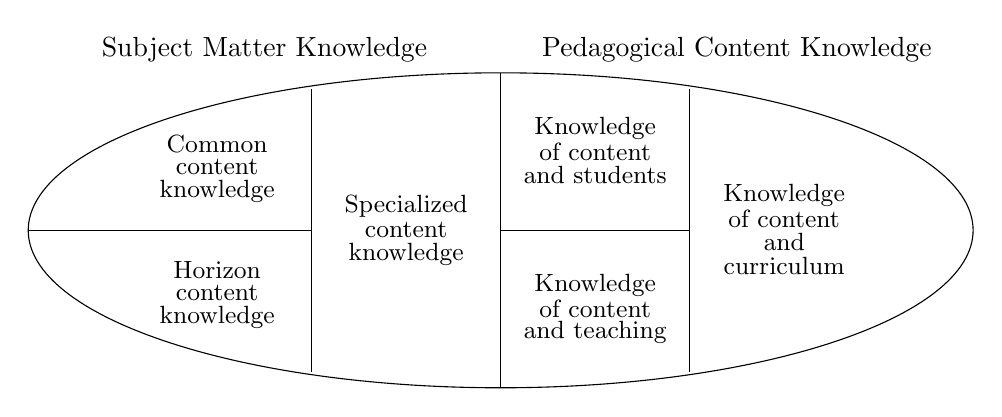
\begin{tikzpicture}
	\draw (0,0) ellipse (6 and 2);
	\draw (-2.4,-1.8) -- (-2.4,1.8);
	\draw (2.4, -1.8) -- (2.4,1.8);
	\draw (0,-2) -- (0,2);
	\draw (-6,0) -- (-2.4, 0);
	\draw (0,0) -- (2.4,0);
	\node at (-1.2,.3) {\small{Specialized}};
	\node at (-1.2,0) {\small{content}};
	\node at (-1.2,-.3) {\small{knowledge}};
	\node at (-3.6,1.1) {\small{Common}};
	\node at (-3.6,.8) {\small{content}};
	\node at (-3.6,0.5) {\small{knowledge}};
	\node at (-3.6,-0.5) {\small{Horizon}};
	\node at (-3.6,-.8) {\small{content}};
	\node at (-3.6,-1.1) {\small{knowledge}};
	\node at (1.2,1.3) {\small{Knowledge}};
	\node at (1.2,1) {\small{of content}};
	\node at (1.2,.7) {\small{and students}};
	\node at (1.2,-.7) {\small{Knowledge}};
	\node at (1.2,-1) {\small{of content}};
	\node at (1.2,-1.3) {\small{and teaching}};
	\node at (3.6,.45) {\small{Knowledge}};
	\node at (3.6,.15) {\small{of content}};
	\node at (3.6,-.15) {\small{and}};
	\node at (3.6,-.45) {\small{curriculum}};
	\node at (-3,2.3) {Subject Matter Knowledge};
	\node at (3,2.3) {Pedagogical Content Knowledge};
\end{tikzpicture}
\end{document}